\section{Chapter7: Independece}

\subsection{Definition}

\begin{exercise}\label{7.1.3}
7.1.3. Show that a collection of events $\{ A_i\}_{i \in I}$ are independent if and only if for any finite $J \subseteq I$,
$$
    \mathbb{P}(\bigcap_{j \in J} A_j)  = \prod_{j \in J} A_j. 
$$
\end{exercise}
\begin{answer} (Neng-Tai)
    For any $B_i \in \{ A_i, A_i^c\}$. Where $j \in J$ finite index, $|J| = m+n \in \mathbb{N}$. Let $J = J_1 \bigcup J_2$, where $J_1 = \{ j | B_j = A_j\}, J_2 = \{ j| B_j = A_j^c\}$, and $|J_1| = m, |J_2| = n$, 
    
    \begin{equation*}
        \begin{aligned}
            \mathbb{P}(\bigcap_{j \in J} B_j) &= \mathbb{P}(\bigcap_{j \in J_1} A_j \cap \bigcap_{j \in J_2} A_j^c) = \mathbb{P}(\bigcap_{j \in J_1} A_j \cap (\Omega \textbackslash \bigcup_{j \in J_2}A_j)) 
            \\ &= \mathbb{P}(\bigcap_{j \in J_1} A_j) - \mathbb{P}(\bigcap_{j \in J_1} A_j \cap(\bigcup_{j \in J_2}A_j )) \hspace{2.5cm} \text{(Disjoint additivity)} 
            \\ &= \prod_{j \in J_1} \mathbb{P}(A_j) - \mathbb{P}(\bigcup_{k \in J_2} (A_k \bigcap_{j \in J_1} A_j))
            \\ & = \prod_{j \in J_1} \mathbb{P}(A_j) - \left[ \sum\limits_{l = 1}^n \sum\limits_{ \{ j_1,\dots, j_l \} \subseteq J_2} (-1)^{l-1}\mathbb{P}((\bigcap_{j \in  \{ j_1,\dots, j_l \}} A_j) \cap \bigcap_{j \in J_1} A_j) \right]  \\&\qquad \qquad \qquad \qquad \qquad \qquad \qquad  \text{(Includsion-exclusion principle)}
            \\ &= \prod_{j \in J_1} \mathbb{P}(A_j) \left[ 1 - \sum\limits_{l = 1}^n \sum\limits_{ \{ j_1,\dots, j_l \} \subseteq J_2} (-1)^{l-1}\prod_{j \in  \{ j_1,\dots, j_l \}}\mathbb{P}(A_j)  \right]  
            \\ &= \prod_{j \in J_1} \mathbb{P}(A_j) \prod_{j \in J_2} (1 - \mathbb{P}(A_j)) = \prod_{j \in J} \mathbb{P}(B_j)  && 
        \qquad \qed
        \end{aligned}
    \end{equation*}
\end{answer}
\begin{exercise} \label{7.1.5}
7.1.5. Let $\{ X_n \}_{n=1}^{ \infty }$ be a sequence of random variables defined on the same probability space. If $X_n$ is independent of $\sigma (X_1,..., X_n )$ for each $n$, prove that the whole collection is independent.
\end{exercise}
\begin{answer}
    7.1.5. (Neng-Tai) 
    \\Need to show:
    \\For any finite $J \subseteq \mathbb{N}$,
    $\mathbb{P}(\bigcap_{i \in J }B_{i} ) = \prod_{i \in J} \mathbb{P}(B_i)$, where $B_{i} \in \sigma(X_i)$.
    \\ To show this, we perform induction on the cardinality of $J$.
    \\For $|J| = 2 $, let $J = \{ i_1, i_2 \},$ where $i_2 > i_1 \geq 1 $. Since $\sigma (X_{i_2})$ and $\sigma (X_{1}, X_{2}, ... ,X_{i_1},...,X_{i_2 - 1} )$ are independent, and observe that $\sigma (X_{i_1}) \subseteq \sigma (X_{1}, X_{2}, ... ,X_{i_1},...,X_{i_2 - 1} ))$, 
    \\given any $B_{i_2} \in \sigma(X_{i_2})$ and $B_{i_1} \in \sigma(X_{i_1})\subseteq \sigma (X_{1}, X_{2}, ... ,X_{i_1},...,X_{i_2 - 1} ))$,
    \\we have $\mathbb{P}(B_{i_1} \cap B_{i_2} ) = \mathbb{P}(B_{i_1}) \mathbb{P}(B_{i_2})$.
    \\Suppose the statement holds for $|J| = n$, where $n 	\geq 2$.
    \\For $|J| = n+1 $, let $J = \{ i_1, i_2,...,i_{n+1} \},$ where $1 \leq i_1 < i_2< ...< i_{n+1}$.
    \\Given  any $B_{i_k} \in \sigma(X_{i_k})$, where $k \in \{1,...,n+1\}$, observe that:
    \begin{equation*}
        B_{i_k} \in \sigma (X_{i_k}) \subseteq \sigma (X_{1}, X_{2},...,X_{i_{n+1} - 1} ), \forall k \in \{ 1,...,n \} \Longrightarrow \bigcap^{n}_{k =1}B_{i_k} \in \sigma (X_{1}, X_{2},...,X_{i_{n+1} - 1} ).
    \end{equation*}
    \\Since $\sigma (X_{i_{n+1}})$ and $\sigma (X_{1}, X_{2},...,X_{i_{n+1} - 1} )$ are independent sub $\sigma - $ algebras, 
    \\$\Longrightarrow \mathbb{P}(\bigcap^{n}_{k =1}B_{i_k} \cap B_{i_{n+1}} ) = \mathbb{P}(\bigcap^{n}_{k =1}B_{i_k}) \mathbb{P}(B_{i_{n+1}})$,
    \\By induction hypothesis, the statement holds for $|J| = n$, hence $\mathbb{P}(\bigcap^{n}_{k =1}B_{i_k}) = \prod^n_{k=1} \mathbb{P}(B_{i_k}) $
    \\$\Longrightarrow \mathbb{P}(\bigcap^{n+1}_{k =1}B_{i_k} ) = \prod^{n+1}_{k=1} \mathbb{P}(B_{i_k})$. \qquad \qed
\end{answer}

\begin{exercise}7.1.6. If $X_1,\cdots, X_n$ are independent random variables and $f:\mathbb{R}^n\mapsto\mathbb{R}$ is a measurable function, show that the law of $f(X_1,\cdots, X_n)$ is determined by the laws of $X_1,\cdots, X_n$.
\end{exercise}

\begin{answer}
    First I show that the law of $(X_1,\cdots,X_n)$ can be determined by the law of $X_i$. Let $\mu$ be the law of $(X_1,\cdots,X_n)$, and let $\mu_i$ be the law of $X_i$. Then for any $A_1\times\cdots\times A_n$ where $A_i\in\mathcal{B}(\mathbb{R})$,
    \begin{equation*}
        \begin{aligned}
            \mu(A_1\times\cdots\times A_n)&=\mathbb{P}\big(\{(X_1,\cdots,X_n)\in A_1\times\cdots\times A_n\}\big) \\
            &=\mathbb{P}\Big(\bigcap^n_{i=1}\{X_i\in A_i\}\Big) \\
            &= \prod^n_{i=1}\mathbb{P}\big(\{X_i\in A_i\}\big) && \text{(By independence of $X_i$s)} \\
            &=\prod^n_{i=1}\mu_i(A_i) && \text{(law of $X_i$s)}\\
            &=\mu_1\times\cdots\times\mu_n(A_1\times\cdots\times A_n),
        \end{aligned}
    \end{equation*}
    where $\mu_1\times\cdots\times\mu_n$ is a measure on $(\mathbb{R}^n, \mathcal{F})$ that agrees with $\prod^n_{i=1}\mu_i(A_i)$ on the set $\mathcal{P} = \{A_1\times\cdots\times A_n:A_i\in\mathcal{B}(\mathbb{R})\}$. (It exists by Proposition 3.1.1.)\\
    Since $\mathcal{P}$ is closed under finite intersection, it is a $\pi$-system. Also, there is a sequence of subsets $\{\mathbf{A}_n\}_{n\in\mathbb{N}}$ in $\mathcal{P}$ increasing to $\mathbb{R}^n$. Hence by Theorem 1.3.6, $\mu=\mu_1\times\cdots\times\mu_n$ on $\sigma(\mathcal{P})=\mathcal{F}$ since they agree on $\mathcal{P}$. Hence the law of $(X_1,\cdots,X_n)$ is exactly the product measure $\mu_1\times\cdots\times\mu_n$.\\
    Since $f:\mathbb{R}^n\rightarrow\mathbb{R}$ is measurable, the law of $f(X_1,\cdots,X_n)$, $\nu$, can be wrote as
    \begin{equation*}
        \begin{aligned}
                    \nu(S) &= \mathbb{P}(\{f(X_1,\cdots,X_n)\in S\}) \\
                    &= \mathbb{P}\big(\big\{(X_1,\cdots,X_n)\in \{f\in S\}\big\}\big) \\
                    &= \mu(\{f\in S\}) \\
                    &= \mu_1\times\cdots\times\mu_n(\{f\in S\}).
        \end{aligned}
    \end{equation*}
    for any $S\in\mathcal{B}(\mathbb{R})$. 
        \qquad \qed

\end{answer}
\begin{exercise} 7.1.7. 
If $\{ X_i\}_{i \in I}$ is a collection of independent random variables and $\{A_i \}_{i \in I}$ is a collection of measurable subsets of $\mathbb{R}$, show that the events $\{X_i \in A_i\}_{i_ \in I}$ are independent. 
\end{exercise}

\begin{answer}
    (Hao) \\
    A random variable is a measurable function, and $A_i \in B(\mathbb{R})$, so the pullback of $A_i$ will be in the $\sigma(X_i)$, i.e $\sigma(X_i^{-1}(A_i)) \subset \sigma(X_i)$. Hence the statement is a direct implication that $\{ \sigma(X_i) \}$ are independent based on the assumption. \qquad \qed
\end{answer}

\begin{exercise}
    7.1.8. If $\{ F_i\}_{i \in I}$ is a family of cumulative distribution functions, show that there is a probability space $(\Omega ,\mathcal{F}, \mathbb{P} )$ and independent random variables $\{ X_i\}_{i \in I}$ defined on $\Omega$ such that for each $i$, $F_i$ is the C.D.F. of $X_i$.(Hint: use product spaces.)
\end{exercise}
\begin{answer}
    7.1.8(Neng-Tai)
    \\For any $i \in I$, let $\Omega_{i} = (0,1)$, $\mathcal{B}_i = $ the restriction of $\mathcal{B}(\mathbb{R})$ to $(0,1)$ and $\lambda_{i}$ be the restriction of Lebesgue measure to $(0,1)$, then $(\Omega_i, \mathcal{B}_i, \lambda_i)$ is a probability space.
    \\For $\omega \in \Omega_i$, define $Y_{i}(\omega) \coloneqq$ inf $\{ t \in \mathbb{R} : F_{i}(t)\geq \omega\}$, where $F_{i} { } 's$ are the given cumulative distribution functions. By Proposition 5.2.2, $\forall i \in I, Y_i$ is measurable and $F_i$ is the C.D.F of $Y_i \Longrightarrow F_{i}(t) = \lambda_{i}(Y_{i}(\omega) \leq t)$.
    \\Set $\Omega = \prod_{i \in I}\Omega_i$, and the product $\sigma $-algebra be $\mathcal{F} = \prod_{i \in I} \mathcal{B}_i$, then exist a unique probability measure $\mathbb{P} = \prod_{i \in I} \lambda_i$ on $(\Omega, \mathcal{F})$.
    \\Now we will begin to construct the required independent random variables $X_i$. Let $p_i: \Omega \rightarrow \Omega_i$ be the canonical projection defined by $p_i(\omega) \coloneqq \omega_i$, where $\omega = \prod_{j \in I}\omega_j$. Observe that for any $\omega_i \in \mathcal{B}_i$, $p_{i}^{-1}(\omega_i) = \prod_{j \in I \setminus \{ i\}} \Omega_j \times \omega_i \in \mathcal{F}$, hence $p_i$ is measurable.
    \\Then we can define $X_i: \Omega \rightarrow \mathbb{R}$ by $X_i(\omega) \coloneqq Y_{i} \circ p_{i}(\omega) \Longrightarrow X_i$ is measurable.
    \\
    \\Claim: $F_i$ is the C.D.F of $X_i$.
    \\Proof. Let $G_i(t)$ be the C.D.F of $X_i$, then
    \begin{equation*}
        \begin{aligned}
            G_i(t) &= \mathbb{P}(X_i(\omega) \leq t)
            =\mathbb{P}(p_{i}^{-1} \circ Y_{i}^{-1} ( -\infty, t ]) 
            \\&= \mathbb{P}(\prod_{j \in I \setminus \{ i\}} \Omega_j \times Y_{i}^{-1} ( -\infty, t ])
            \\&= \prod_{j \in I \setminus \{ i\}} \lambda_j(\Omega_j) \times \lambda_i(Y_{i}^{-1} ( -\infty, t ])
            \\&= \lambda_i(Y_{i}^{-1} ( -\infty, t ]) = F_i(t)
        \end{aligned}
    \end{equation*}
    $\hfill\Box$
    \\Claim: $X_i$'s are independent random variables.
    \\Proof: Let $J \subseteq I$ be a finite set, $\{ A_i : A_{i} \in \sigma(X_i)\}_{i \in J} \subseteq \Omega$. 
    \\Need to show $\mathbb{P}(\bigcap_{i \in J }A_{i} ) = \prod_{i \in J} \mathbb{P}(A_i)$.
    \\Observe that for any $A_i \in \sigma(X_i)$, $A_i = \prod_{s \in I \setminus \{ i\}} \Omega_s \times \omega_i$, where $\omega_i \in \sigma (Y_i)$.
    \\Hence, 
    \begin{equation*}
        \begin{aligned}
                    \mathbb{P}(\bigcap_{i \in J }A_{i}) &= \mathbb{P}\Big( \bigcap_{i \in J }(\prod_{j \in I \setminus \{ i\}} \Omega_j \times \omega_i)\Big)
                    \\&= \mathbb{P}\Big( (\prod_{s \in I \setminus J}\Omega_s) \times (\prod_{i \in J} \omega_i) \Big)
                    \\&= \Big(\prod_{s \in I \setminus J} \lambda_s(\Omega_s) \Big)\Big( \prod_{i \in J} \lambda_i(\omega_i)\Big) = \prod_{i \in J} \lambda_i(\omega_i)
                    \\&= \prod_{i \in J} \mathbb{P}(\prod_{s \in I \setminus \{ i\}}\Omega_s \times \omega_i) = \prod_{i \in J} \mathbb{P}(A_i)
        \end{aligned}
    \end{equation*}
    $\hfill\qed$ 
\end{answer}

\begin{exercise}7.1.9.
If $\mathcal{A}$ is a $\pi$-system of sets and $B$ is an event such that $B$ and $A$ are independent for every $A\in\mathcal{A}$, show that $B$ and $\sigma(\mathcal{A})$ are independent.
\end{exercise}

\begin{answer}
    $\mathcal{A}$ is a $\pi$-system. B is the set that is independent to all elements in $\mathcal{A}$. \\
    The strategy is to construct a larger $\lambda$-system $\mathcal{L}$ containing $\mathcal{A}$, with its elements are all independent to $B$. Since Dynkin's $\pi-\lambda$ theorem tells us that $\sigma(\mathcal{A})\subset\mathcal{L}$, then the proof would be completed.\\
    Consider the set that collects all the event that is independent to $B$ in $\mathcal{F}$:
    \begin{equation*}
        \mathcal{L}=\{C\in\mathcal{F}:\mathbb{P}(B\cap C)=\mathbb{P}(B)\mathbb{P}(C)\}.
    \end{equation*}
    Check $\mathcal{L}$ is a $\lambda$-system. First $\Omega\in\mathcal{L}$ since $\mathbb{P}(\Omega\cap B)=\mathbb{P}(B)=\mathbb{P}(\Omega)\mathbb{P}(B)$. Secondly if $L\in\mathcal{L}$ then $\mathbb{P}(L\cap B) = \mathbb{P}(B)\mathbb{P}(L)$. Since $\mathbb{P}(L^c\cap B) = \mathbb{P}(B\setminus B\cap L)=\mathbb{P}(B)-\mathbb{P}(B\cap L)$ by $(B\cap L)\cup(B\cap L^c)$ is a disjoint union, we then have $\mathbb{P}(L^c\cap B) = (1-\mathbb{P}(L))\mathbb{P}(B)=\mathbb{P}(L^c)\mathbb{P}(B)$. So $L^c\in\mathcal{L}$. Lastly, suppose $L_1,L_2,\cdots$ is a sequence of disjoint sets in $\mathcal{L}$, then
    \begin{equation*}
        \begin{aligned}
                    \mathbb{P}(\bigcup^\infty_{n=1}L_n\cap B)&=\mathbb{P}(\bigcup^\infty_{n=1}(L_n\cap B)) \\
                    &=\sum_{n\in\mathbb{N}}\mathbb{P}(L_n\cap B) && (\text{$(L_n\cap B)\subset L_n$ and $L_n$s are disjoint}) \\
                    &=\sum_{n\in\mathbb{N}}\mathbb{P}(L_n)\mathbb{P}(B) && (L_n\in\mathcal{L}) \\
                    &=\mathbb{P}(B)\mathbb{P}(\bigcup^\infty_{n=1}L_n) && (L_n\text{  disjoint}).
        \end{aligned}
    \end{equation*}
    So $\mathcal{L}$ forms a $\lambda$-system. Since all the elements $A\in\mathcal{A}$ are independent to $B$, we have $\mathcal{A}\subset\mathcal{L}$.\\
    Now by Dynkin's $\pi-\lambda$ theorem, $\sigma(\mathcal{A})\subset\mathcal{L}$ since $\mathcal{A}$ is a $\pi$-system. Hence $\sigma(\mathcal{A})$ is independent to $B$.
    \qquad \qed
\end{answer}

\begin{exercise}7.1.10. If $\{X_i\}_{i\in I}$ is a collection of independent random variables, then show that for any disjoint subsets $J, K \subseteq I$, the $\sigma$-algebras generated by
$\{X_i\}_{i\in J}$ and $\{X_i\}_{i\in K}$ are independent.
\end{exercise}
\begin{answer}
    $\{X_i\}_{i\in I}$ is a collection of independent random variables. Let $J,K\subseteq I$ be disjoint. I want to show that $\sigma(\{X_i\}_{i\in J})$ and $\sigma(\{X_i\}_{i\in K})$ are independent.\\
    Define $\mathcal{P}_J$, $\mathcal{P}_K$ as follows:
    \begin{equation*}
        \begin{aligned}
                    &\mathcal{P}_J=\Big\{\bigcap_{i=1}^n\{X_{j_i}\in A_i\}:A_i\in\mathcal{B}(\mathbb{R}), \{j_1,\cdots,j_n\}\subset J\Big\}.\\
                    &\mathcal{P}_K=\Big\{\bigcap_{i=1}^n\{X_{k_i}\in A_i\}:A_i\in\mathcal{B}(\mathbb{R}), \{k_1,\cdots,k_n\}\subset K\Big\}.
        \end{aligned}
    \end{equation*}
    They're $\pi$-systems since the intersection is closed in $\mathcal{P}_J$ ($\mathcal{P}_K$):
    \begin{equation*}
        \left(\bigcap_{n=1}^{N_1}\{X_{i_n}\in A_n\}\right)\bigcap\left(\bigcap_{n=1}^{N_2}\{X_{j_n}\in B_n\}\right)=\bigcap_{n=1}^{N}\{X_{k_n}\in C_n\}
    \end{equation*}
    for some $\{k_1,\cdots,k_N\}\subseteq\{i_1,\cdots,i_{N_1}\}\cup\{j_1,\cdots,j_{N_2}\}$ and some Borel sets $C_n$.\\
    We can also see that $\{X_j\in A\}\in\mathcal{P}_J$ for any $j\in J$ and $A\in\mathcal{B}(\mathbb{R})$, hence
    \begin{equation*}
        \bigcup_{j\in J}\sigma(X_j)=\bigcup_{j\in J}\Big\{\{X_j\in A\}:A\in\mathcal{B}(\mathbb{R})\Big\}\subset\mathcal{P}_J.
    \end{equation*}
    Thus $\sigma(\{X_j\}_{j\in J})\subseteq\sigma(\mathcal{P}_J)$. Similarly $\sigma(\{X_k\}_{k\in K})\subseteq\sigma(\mathcal{P}_K)$.\\
    Let $\cap_{n=1}^{N_1}\{X_{j_n}\in A_n\}\in\mathcal{P}_{J}$ and $\cap_{n=1}^{N_2}\{X_{k_n}\in B_n\}\in\mathcal{P}_{K}$, then by independence of $\{\sigma(X_i)\}_{i\in I}$:
    \begin{equation*}
        \begin{aligned}
                \mathbb{P}\left(\bigcap_{n=1}^{N_1}\{X_{j_n}\in A_n\}\cap\bigcap_{n=1}^{N_2}\{X_{k_n}\in B_n\}\right)&=\prod_{n=1}^{N_1}\mathbb{P}(\{X_{j_n}\in A_n\})\times\prod_{n=1}^{N_2}\mathbb{P}(\{X_{k_n}\in B_n\}) \\
                &=\mathbb{P}\left(\bigcap_{n=1}^{N_1}\{X_{j_n}\in A_n\}\right)\mathbb{P}\left(\bigcap_{n=1}^{N_2}\{X_{k_n}\in B_n\}\right).
        \end{aligned}
    \end{equation*}
    Hence every elements in $\mathcal{P}_J$ are independent to all elements in $\mathcal{P}_K$. By Exercise 7.1.9 this implies $\sigma(\mathcal{P}_J)$ is independent to $\sigma(\mathcal{P}_K)$. Since $\sigma(\{X_j\}_{j\in J})\subseteq\sigma(\mathcal{P}_J)$ and $\sigma(\{X_k\}_{k\in K})\subseteq\sigma(\mathcal{P}_K)$, $\sigma(\{X_j\}_{j\in J})$ is independent to $\sigma(\{X_k\}_{k\in K})$. \qquad \qed
\end{answer}

\begin{exercise} 7.1.11. 
Let $\{X_i\}_{i\in I}$ and $\{Y_j\}_{j\in J}$ be two collections of random variables defined on the same probability space. Suppose that for any finite $F\subseteq I$ and $G\subseteq J$, the collections $\{X_i\}_{i\in F}$ and $\{Y_j\}_{j\in G}$ are independent. Then prove that $\{X_i\}_{i\in I}$ and $\{Y_j\}_{j\in J}$ are independent.
\end{exercise}
\begin{answer}
    $\{X_i\}_{i\in I}$ and $\{Y_j\}_{j\in J}$ are two collections of random variables defined on the same probability space. For any finite $F\subseteq I$ and $G\subseteq J$ the collections $\{X_i\}_{i\in F}$ and $\{Y_j\}_{j\in G}$ are independent. I'm going to prove that $\sigma(\{X_i\}_{i\in I})$ and $\sigma(\{Y_j\}_{j\in J})$ are independent.\\
    Similar to Exercise 7.1.10, define the collection $\mathcal{P}_I$ and $\mathcal{P}_J$ as
    \begin{equation*}
        \begin{aligned}
                    &\mathcal{P}_X=\Big\{\bigcap_{f\in F}\{X_{f}\in A_f\}:A_f\in\mathcal{B}(\mathbb{R}),\,F\subseteq I\Big,\,|F|<\infty\Big\}.\\
                    &\mathcal{P}_Y=\Big\{\bigcap_{g\in G}\{Y_{g}\in A_g\}:A_g\in\mathcal{B}(\mathbb{R}),\,G\subseteq J,\,|G|<\infty\Big\}.
        \end{aligned}
    \end{equation*}
    Then they're $\pi$-systems. Since $\{X_i\in A\}\in\mathcal{P}_X$ for all $A\in\mathcal{B}(\mathbb{R})$ and $i\in I$,
    \begin{equation*}
                \bigcup_{i\in I}\sigma(X_i)=\bigcup_{i\in I}\Big\{\{X_i\in A\}:A\in\mathcal{B}(\mathbb{R})\Big\}\subset\mathcal{P}_X.
    \end{equation*}
    Thus $\sigma(\{X_i\}_{i\in I})\subseteq\sigma(\mathcal{P}_X)$, so does $\sigma(\{Y_j\}_{j\in J})\subseteq\sigma(\mathcal{P}_Y)$.\\
    Let $S_X\in\mathcal{P}_X$, then $S_X=\bigcap_{f\in F}\{X_f\in A_f\}\in\sigma(\{X_f\}_{f\in F})$ for some finite $F\subseteq I$ and some Borel sets $A_f$. If $S_Y\in\mathcal{P}_Y$ we also have $S_Y\in\sigma(\{Y_g\}_{g\in G})$ for some finite $G\subseteq J$. Since $\sigma(\{X_f\}_{f\in F})$ and $\sigma(\{Y_g\}_{g\in G})$ are independent for any finite $F\subseteq I$ and $G\subseteq J$, $S_X$ and $S_Y$ are independent.\\
    Then by Exercise 7.1.9, all elements in $\mathcal{P}_X$ are independent to all elements in $\mathcal{P}_Y$ implies $\sigma(\mathcal{P}_X)$ and $\sigma(\mathcal{P}_Y)$ are independent. Hence $\sigma(\{X_i\}_{i\in I})$ and $\sigma(\{Y_j\}_{j\in J})$ are independent. \qquad \qed
\end{answer}

\subsection{Expectation of a product under independence}

\begin{exercise}7.2.2. \ 
If $X_1, X_2, \dots, X_n$ are independent integrable random variables, show that the product $X_1X_2\cots X_n$ is also integrable and 
$$
    \mathbb{E}(X_1X_2 \cdots X_n) = \mathbb{E}(X_1)\mathbb{E}(X_2)\cdots\mathbb{E}(X_n).
$$
\end{exercise}
\begin{answer} (Hao) \\
    One method is to follow the procedure in the proposition 7.2.1 but do it for $n$ random variables. There is yet another way that we can do this, induction. In order to make induction work, we first have to show that the product of two random variable is still a random variable, so we can make induction w.r.t. the number of random variables $n$. In other words, we first have to show that if $X,Y$ are both measurable function, then $XY$  is also a measurable function. Fortunately, we can refer to exercise 2.1.5 to see that $X+Y$ and $X^2$ are also measurable. Hence
    $$XY = \frac{1}{4}(X+Y)^2 - (X-Y)^2$$ 
    is measurable, i.e $XY$ is a random variable. We can now proceed with the induction.
    
    The base case $n=2$ is shown in the proposition 7.2.1. Suppose the statement of this exercise is correct up to $n = m-1, m \in \mathbb{N}$ (induction hypothesis), and that $X_1X_2 \dots X_{m-1}$ is integrable and is a random variable.
    Then for $n = m$, we may consider the two random variable $X_1X_2 \dots X_{m-1}$ and $X_{m}$. Again, by the proposition 7.2.1 we get the result that $X_1X_2\dots X_m$ is also integrable and 
    $$\mathbb{E}(X_1X_2 \dots X_m) = \mathbb{E}(X_1X_2 \dots X_{m-1}) \mathbb{E}(X_m) =  \mathbb{E}(X_1)\mathbb{E}(X_2)\cdots\mathbb{E}(X_n).$$
    The first equality works because we treat $X_1X_2 \dots X_{m-1}$ as one integrable random variable; the second equality works because of our induction hypothesis.
    
    Hence, the statement of this exercise is true for all $n \in \mathbb{N}$.
\end{answer} \qed \qquad

\begin{exercise} 7.2.3. If $X$ and $Y$ are independent integrable random variables, show that Cov$(X, Y ) = 0$. In other words, independent random variables are
uncorrelated.
\end{exercise}

\begin{answer} Suppose $X,Y$ are two independent random variables on the same probability space, then $\mathbb{E}\big((X-\mathbb{E}X)(Y-\mathbb{E}Y)\big)=\mathbb{E}(XY-X\mathbb{E}(Y)-Y\mathbb{E}(X)+\mathbb{E}(X)\mathbb{E}(Y))=0$ since $\mathbb{E}(XY)=(\mathbb{E}X)(\mathbb{E}Y)$ by independence.
\end{answer}\qed \qquad

\begin{exercise} 7.2.4 \\
Give an example of a pair of uncorrelated random variables that are not independent.
\end{exercise}
\begin{answer} (Hao) \\
Set $X \sim \text{Unif}[-1,1],\  Y = X^2$. Then,
$$\mathbb{E}(XY) = \mathbb{E}(X^3) = \int_{-1}^{1}x^3\frac{1}{2}dx = 0 = 0 \cdot \frac{2}{3} =  (\int_{-1}^{1} x dx) \cdot (\int_0^1 y\frac{1}{\sqrt{y}} dy) = \mathbb{E}(X)\mathbb{E}(Y)$$
However, $X$ and $Y$ are clearly not independent because 
$$\mathbb{P}(X \in [-0.5,0.5], Y \in [1/\sqrt{2},1]) = 0 \neq \frac{1}{2} \cdot 1 = \mathbb{P}(X \in [-0.5,0.5]) \mathbb{P}(Y \in [1/\sqrt{2},1])$$
\end{answer}\qed \qquad

\begin{exercise}7.2.5 \ 
    Give an example of three random variables $X_1, X_2, X_3$ that are pairwise independent but not independent.
\end{exercise}
\begin{answer}(Hao) \\
    \begin{figure}[!h]
        \centering
        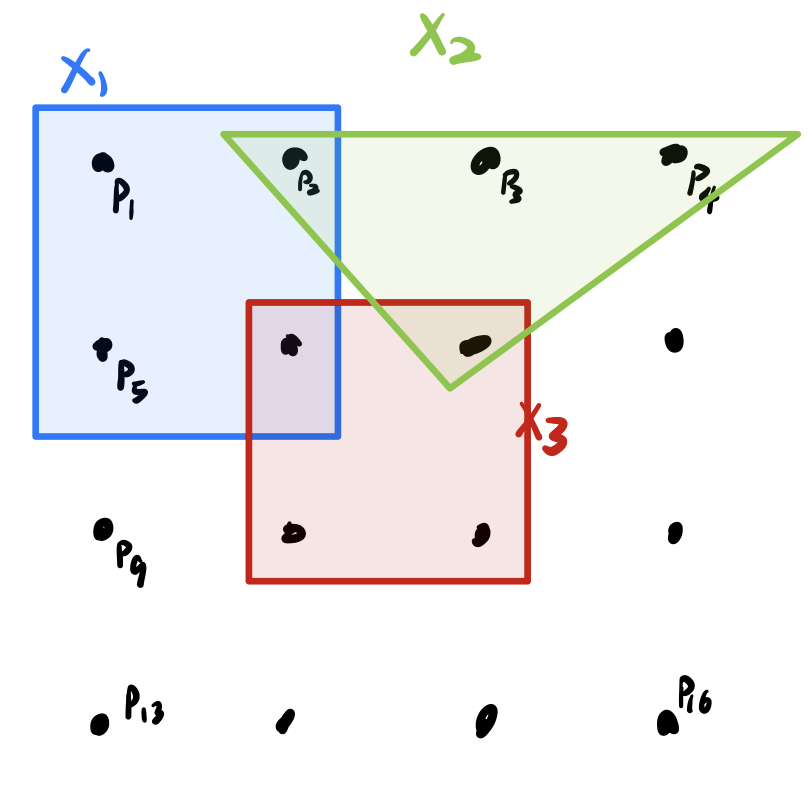
\includegraphics[width=\textwidth/3]{Note/Figures/7.2.5.png}
        \caption{An example that is pairwise independent but not independent}
    \end{figure}
    
    The example is an discrete probability space,
    $\Omega = \{p_i\}_{i=1}^{16}$, $\mathcal{F} = \sigma(\Omega)$. The probability measure is $\mathbb{P}(A) = \frac{||A||}{16}$. In other words, counting how much points $p_i$ are selected. 
    Let's define 
    \begin{equation*}
        \begin{aligned}
            X_1 &= 1_{ \{p_1,p_2,p_5,p_6 \} } \\
            X_2 &= 1_{ \{p_2,p_3,p_4,p_6 \} } \\
            X_3 &= 1_{ \{p_6,p_7,p_{10},p_{11} \} } 
        \end{aligned}
    \end{equation*}
    From exercise \ref{7.1.3}, we know that we only have to check the case with $A_i = \{ X_i = 1\}$. For example, we take $X_1$ and $X_2$
    $$
        \mathbb{P}(X_1 = 1 \cap X_2 = 1) = \mathbb{P}(\{p_2\}) = \frac{1}{16} = (\frac{1}{4})^2 \mathbb{P}(X_1 = 1 )\mathbb{P}( X_2 = 1)
    $$
    Hence, $\{ X_i\}_{i=1}^3$ is pairwise independent. However, the collection $\{ X_i\}_{i=1}^3$ is not independent because
    $$\mathbb{P}(\bigcap\limits_{i=1}^3 X_i = 1) = 0 \neq (\frac{1}{4})^3 = \prod\limits_{i=1}^3 \mathbb{P}( X_i = 1)$$
    
    
\end{answer}\qed \qquad

\subsection{The second Borel-Cantelli lemma}

\subsection{The Kolmogorov zero-one law}
\begin{exercise}7.4.2.
If $\mathcal{G}$ is a trivial $\sigma$-algebra for a probability measure $\mathbb{P}$, show that any random variable $X$ that is measurable with respect to $\mathcal{G}$ must be equal to a constant almost surely.
\end{exercise} 
\begin{answer}Since $\mathbb{P}\big(\cup_{n\in\mathbb{Z}}\{X\in(n,n+1]\}\big)=\sum_{n\in\mathbb{N}}\mathbb{P}(X\in(n,n+1])=1$ and $X$ is $\mathcal{G}$-measurable, there is a unique integer $m$ s.t. $\mathbb{P}(X\in(m,m+1])=1$. Set $I_1=(m,m+1]$, construct $I_k$ for $k\geq 2$ by following: suppose $I_{k-1}=(a,b]$,  

\end{answer}\qed \qquad
\begin{exercise}7.4.3.
 If $\{ X_n\}_n^\infty$ is a sequence of independent random variables, show that the random variables $\limsup X_n$ and $\liminf X_n$ are equal to constants almost surely.
\end{exercise}
\begin{answer} \\
Let $a\in\mathbb{R}$. Since $\bigcup_{k\geq n}\{X_k>a\}$ decreases as $n\rightarrow\infty$,
\begin{equation*}
    \begin{aligned}
        \Big\{\limsup_{n\rightarrow\infty}X_n>a\Big\}=\bigcap_{n\in\mathbb{N}}\bigcup_{k\geq n}\{X_k>a\}=\bigcap_{n\geq N}\bigcup_{k\geq n}\{X_k>a\}\hspace{0.25cm}\forall N\in\mathbb{N}.
    \end{aligned}
\end{equation*}
Hence $\{\limsup_{n\rightarrow\infty}X_n>a\}\in\sigma(X_N,X_{N+1},\cdots)$ for all $N\in\mathbb{N}$. That is, $\limsup_{n\rightarrow\infty}X_n$ is $\bigcap_{n\in\mathbb{N}}\sigma(X_n,X_{n+1},\cdots)$-measurable. Therefore by \textsc{Exercise 7.4.2}, $\limsup_{n\rightarrow\infty}X_n$ equals a constant almost surely. For $\liminf_{n\rightarrow\infty}X_n$, since $\bigcup_{k\geq n}\{X_k<a\}$ decreases as $n\rightarrow\infty$,
\begin{equation*}
    \Big\{\liminf_{n\rightarrow\infty}X_n<a\Big\}=\bigcap_{n\in\mathbb{N}}\bigcup_{k\geq n}\{X_k<a\}=\bigcap_{n\geq N}\bigcup_{k\geq n}\{X_k<a\}\hspace{0.25cm}\forall N\in\mathbb{N}.
\end{equation*}
Then the same reason holds. Hence $\liminf_{n\rightarrow\infty}X_n$ equals a constant almost surely, too.
\end{answer}\qed\qquad


\begin{exercise}7.4.4.
Let $\{X_n\}^\infty_{n=1}$ be a sequence of independent random variables. Let $S_n := X_1 +\cdots+ X_n$, and let $\{a_n\}^\infty_{n=1}$ be a sequence of constants increasing to infinity. Then show that $\limsup S_n/a_n$ and $\liminf S_n/a_n$ are constants almost surely.
\end{exercise}
\begin{answer}
$Proof.$ Let $S_{k+1,n}=\sum_{i=k+1}^n X_i$, denote $S_{1,k}=S_k$. Claim:
\begin{equation*}
    \limsup_{n\rightarrow\infty}\frac{S_n}{a_n}=\limsup_{n\rightarrow\infty}\frac{S_{k+1,n}}{a_n}\hspace{0.5cm}\text{and}\hspace{0.5cm}\liminf_{n\rightarrow\infty}\frac{S_n}{a_n}=\liminf_{n\rightarrow\infty}\frac{S_{k+1,n}}{a_n}
\end{equation*} for any $k\in\mathbb{N}$.\\
(Proof of claim) Let $k\in\mathbb{N}$. Since $a_n$ increases to infinity, there is a sufficiently large $N>k$ s.t. $a_n>0\;\forall n\geq N$. Suppose $S_{k}=\sum_{i=1}^k X_i\geq 0$, then for any $m\geq n\geq N$,
\begin{equation*}
    \begin{aligned}
        &\frac{S_m}{a_m}\leq\frac{S_{1,k}}{a_n}+\frac{S_{k+1,m}}{a_m}
        %&\frac{S_m}{a_m}=\frac{S_{1,k}}{a_m}+\frac{S_{k+1,m}}{a_m}\geq\frac{S_{k+1,m}}{a_m}\\
    \end{aligned}
\end{equation*}
Hence
\begin{equation*}
    \begin{aligned}
        \sup_{m\geq n}\Big\{\frac{S_m}{a_m}\Big\}\leq\frac{S_{k}}{a_n}+\sup_{m\geq n}\Big\{\frac{S_{k+1,m}}{a_m}\Big\}\text{ and }\inf_{m\geq n}\Big\{\frac{S_m}{a_m}\Big\}\leq\frac{S_{k}}{a_n}+\inf_{m\geq n}\Big\{\frac{S_{k+1,m}}{a_m}\Big\}.
    \end{aligned}
\end{equation*}
Take $n\rightarrow\infty$. Since $a_n\uparrow\infty$, $S_k/a_n\downarrow 0$. Thus
\begin{equation*}
    \begin{aligned}
        \limsup_{n\rightarrow\infty}\frac{S_n}{a_n}\leq\limsup_{n\rightarrow\infty}\frac{S_{k+1,n}}{a_n}\text{ and }\liminf_{n\rightarrow\infty}\frac{S_n}{a_n}\leq\liminf_{n\rightarrow\infty}\frac{S_{k+1,n}}{a_n}.
    \end{aligned}
\end{equation*}
For the other direction, since $a_m > 0$ when $m\geq N$,
\begin{equation*}
    \frac{S_m}{a_m}=\frac{S_k}{a_m}+\frac{S_{k+1,m}}{a_m}\geq\frac{S_{k+1,m}}{a_m}
\end{equation*}
Thus we have
\begin{equation*}
    \begin{aligned}
        \limsup_{n\rightarrow\infty}\frac{S_n}{a_n}\geq\limsup_{n\rightarrow\infty}\frac{S_{k+1,n}}{a_n}\text{ and }\liminf_{n\rightarrow\infty}\frac{S_n}{a_n}\geq\liminf_{n\rightarrow\infty}\frac{S_{k+1,n}}{a_n}.
    \end{aligned}
\end{equation*}
Hence the claim holds for $S_k\geq 0$.

If $S_{k}<0$, then we can check for any $m\geq n\geq N$,
\begin{equation*}
    \begin{aligned}
        &\frac{S_m}{a_m}\geq\frac{S_{k}}{a_n}+\frac{S_{k+1,m}}{a_m};\\
        &\frac{S_m}{a_m}=\frac{S_{k}}{a_m}+\frac{S_{k+1,m}}{a_m}\leq\frac{S_{k+1,m}}{a_m}\\
    \end{aligned}
\end{equation*}
Then repeat the process we still have the same conclusion. $\square$
\\
With this fact, we have
\begin{equation*}
    \begin{aligned}
        &\Big\{\limsup_{n\rightarrow\infty}\frac{S_n}{a_n}>a\Big\}=\bigcap_{k\in\mathbb{N}}\Big\{\limsup_{n\rightarrow\infty}\frac{S_{k+1,n}}{a_n}>a\Big\}\\
        &\Big\{\liminf_{n\rightarrow\infty}\frac{S_n}{a_n}<a\Big\}=\bigcap_{k\in\mathbb{N}}\Big\{\liminf_{n\rightarrow\infty}\frac{S_{k+1,n}}{a_n}<a\Big\}
    \end{aligned}
\end{equation*}
Check: $\limsup_{n\rightarrow\infty}S_{k+1,n}/a_n$ is $\sigma(X_k,X_{k+1},\cdots)$-measurable.\\
For any $n> k$, $S_{k+1,n}=f(X_{k+1},\cdots,X_n)$ where $f:(x_1,\cdots,x_{n-k})\mapsto x_1+\cdots+x_{n-k}$. Since $f$ is continuous and thus measurable, by \textsc{Exercise 5.1.1.} we know that $S_{k+1,n}$ is $\sigma(X_{k+1},\cdots,X_n)$-measurable, and thus $\sigma(X_{k+1},\cdots)$-measurable. This implies that $\limsup_{n\rightarrow\infty}S_{k+1,n}/a_n$ is $\sigma(X_k,X_{k+1},\cdots)$-measurable.\\
Hence
\begin{equation*}
    \Big\{\limsup_{n\rightarrow\infty}\frac{S_n}{a_n}>a\Big\}\in\bigcap_{k\in\mathbb{N}}\sigma(X_k,X_{k+1},\cdots)=\mathcal{T}.
\end{equation*}
Since $\mathcal{T}$ is a trivial sigma algebra and $\limsup_{n\rightarrow\infty}S_n/a_n$ is $\mathcal{T}$-measurable, $\limsup_{n\rightarrow\infty}S_n/a_n$ is a constant almost surely by \textsc{Exercise 7.4.2}. 
\end{answer}\qquad \qed

\subsection{Zero-one laws for i.i.d. random variables}

\begin{exercise}7.5.5.
Suppose that we have $m$ boxes, and an infinite sequence of
balls are dropped into the boxes independently and uniformly at random. Set this
up as a problem in measure-theoretic probability, and prove that with probability
one, each box has the maximum number of balls among all boxes infinitely often.
\end{exercise}
$Proof.$ Let $\Omega=\{1,\cdots,m\}^\mathbb{N}$ be the sample space. Define the random variables $\{X_n\}_{n\in\mathbb{N}}$ on $\Omega$ such that $X_n(\omega)=\omega(n)=\omega_n$ for all $\omega$ and $n$. (Simply $\{X_n\}_{n\in\mathbb{N}}(\omega)=\omega$)\\
Set $k\in[m]$, and consider the subset $E\subseteq\Omega$:
\begin{equation*}
    E=\bigcap_{N\in\mathbb{N}}\bigcup_{n\geq N}\{\omega\in\Omega:k\text{ is the maximal appearance in }(\omega_1,\cdots,\omega_n)\},
\end{equation*}
and denotes the event $E_n=\{\omega\in\Omega:k\text{ is the maximal appearance in }\omega_1,\cdots,\omega_n\}$.

Since $E = \bigcap_{N\geq M}\bigcup_{n\geq N}E_n$ for any $M\in\mathbb{N}$, $E$ is permutation invariant. Hence if we define $f=\mathds{1}_E$, then $\mathds{1}_E\big((\omega_i)_{i\in\mathbb{N}}\big)=\mathds{1}_E\big((\omega_{\sigma(i)})_{i\in\mathbb{N}}\big)$ since $\omega\in E$ is equivalent to $\omega_{\sigma(i)}_{i\in\mathbb{N}}\in E$ for any permutation $\sigma$. This also means $f(\{X_i\}_{i\in\mathbb{N}})=f(\{X_{\sigma(i)}\}_{i\in\mathbb{N}})$ on $\Omega$, then by \textsc{Corollary 7.5.4}, $f(\{X_i\}_{i\in\mathbb{N}})$ is a constant almost surely.

Since $\{f(X_1,X_2,\cdots)=1\}=\{(X_1(\omega),X_2(\omega),\cdots)\in E\}=E$, $\mathbb{P}(E)\in\{0,1\}$. Moreover, since $\mathbb{P}\Big(\bigcup_{n\geq N} E_n\Big)\geq\mathbb{P}(E_N)$ for any  $N\in\mathbb{N}$, and
\begin{equation*}
    \begin{aligned}
        \mathbb{P}(E_N)&=\mathbb{P}\big(\{\omega\in\Omega:k\text{ is the maximal appearance in }(\omega_1,\cdots,\omega_N)\}\big)\\
        &= 1-\mathbb{P}\Big(\bigcup_{l\neq k}\{\omega:l\text{ is the maximal appearance in }(\omega_1,\cdots,\omega_N)\}\Big)\\
        &\geq 1-\sum_{l\neq k}\mathbb{P}\big(\{\omega:l\text{ is the maximal appearance in }(\omega_1,\cdots,\omega_N)\}\big)\\
        &=1-(m-1)\mathbb{P}(E_N),
    \end{aligned}
\end{equation*}
we have $\mathbb{P}\Big(\bigcup_{n\geq N} E_n\Big)\geq\mathbb{P}(E_N)\geq 1/m$ for any $N$.\\
Hence $\mathbb{P}(E)=\lim_{N\rightarrow\infty}\mathbb{P}\Big(\bigcup_{n\geq N}E_n\Big)\geq 1/m\neq 0$, i.e. $\mathbb{P}(E)=1$. So this event happens with probability one. \qed \qquad

\subsection{Random vectors}
\begin{exercise}7.6.1.
Prove that the c.d.f. of a random vector uniquely characterizes its law.
\end{exercise}
$Proof.$ Claim that $\mathcal{R}=\{(-\infty,b_1]\times\cdots\times(-\infty,b_n]:b_i\in\mathbb{R}\}$ generates $\mathcal{B}_{\mathbb{R}^n}$. Since $\mathcal{B}_{\mathbb{R}^n}=\sigma\big(\big\{\{x\in\mathbb{R}^n:x_i\in E\}:E\in\mathcal{B}_\mathbb{R},i\in[n]\big\}\big)$, it's clear that $\sigma(\mathcal{R})\subseteq\mathcal{B}_{\mathbb{R}^n}$. For the other direction, since the collection $\{(-\infty,b]:b\in\mathbb{R}\}$ generates $\mathcal{B}_\mathbb{R}$, for any $i\in[n]$ and $E\in\mathcal{B}_{\mathbb{R}^n}$ we have $\{x_i\in E\}\in\sigma\big(\big\{\{x_i\in(-\infty,b_i]\}:b_i\in\mathbb{R}\big\}\big)$, and thus $\{x_i\in E\}\in\sigma(\mathcal{R})$. Therefore, $\mathcal{B}_{\mathbb{R}^n}\subseteq\sigma(\mathcal{R})$.

Suppose $X,Y$ are two random vectors that have the same c.d.f $F$, then $\mu_X=\mu_Y$ on $\mathcal{R}$. Since $\mathcal{R}$ is a $\pi$-system (it's closed under finite intersection), by \textsc{Theorem 1.3.6} we have $\mu_X=\mu_Y$ on $\sigma(\mathcal{R})=\mathcal{B}_{\mathbb{R}^n}$. Hence the law corresponding to $F$ is unique. \qed \qquad

\begin{exercise}7.6.2. If $X_1,\cdots, X_n$ are independent random variables with laws $\mu_1,\cdots,\mu_n$, then show that the law of the random vector $(X_1,\cdots, X_n)$ is the product measure $\mu_1\times\cdots\times\mu_n$.
\end{exercise}
\begin{answer}
    Let $\mu$ be the law of random vector $(X_1,\cdots,X_n)$. Let $\mathcal{R}=\{E_1\times\cdots\times E_n:E_i\in\mathcal{B}_\mathbb{R}\}$. Since $X_1,\cdots,X_n$ are independent,
\begin{equation*}
\begin{aligned}
    \mu(E_1\times\cdots\times E_n)&=\mathbb{P}(X_1\in E_1,\cdots, X_n\in E_n)\\&
    =\prod_{i=1}^n\mathbb{P}(X_i\in E_i)\\&
    =\prod_{i=1}^n\mu_i(E_i)=\mu_1\times\cdots\times\mu_n(E_1\times\cdots\times E_n).
\end{aligned}
\end{equation*}
Hence $\mu$ and $\mu_1\times\cdots\times\mu_n$ agrees on $\mathcal{R}$. Since $\mathcal{R}$ is a $\pi$-system that generates $\mathcal{B}_{\mathbb{R}^n}$, by \textsc{Theorem 1.3.6}, $\mu=\mu_1\times\cdots\times\mu_n$ on $\mathcal{B}_{\mathbb{R}^n}$. Therefore $\mu_1\times\cdots\times\mu_n$ is the law of $(X_1,\cdots,X_n)$.
\end{answer}\qed \qquad

\begin{exercise}7.6.3. If $X_1,\cdots, X_n$ are independent random variables, show that
the cumulative distribution function and the characteristic function of the random
vector $(X_1,\cdots, X_n)$ can be written as products of one-dimensional distribution
functions and characteristic functions.
\end{exercise}
\begin{answer}
    Let $F_i$ be the c.d.f of $X_i$ and $F$ be the c.d.f of random vector $(X_1,\cdots,X_n)$. Since $X_1,\cdots,X_n$ are independent, by \textsc{Exercise 7.6.2} we have $F(x_1,\cdots,x_n)=\mu_1\times\cdots\times\mu_n((-\infty,x_1]\times\cdots\times(-\infty,x_n])=\prod_{i=1}^n\mu_i((-\infty,x_i])=\prod_{i=1}^nF_i(x_i)$.

Claim: If $X_1,\cdots,X_n$ are independent, let $t\in\mathbb{R}$, then the complex-valued random variables $\{Y_k=\exp(itX_k)\}_{k=1}^n$ are independent.\\
(Proof of Claim) Since $x\mapsto\exp(itx)$ is continuous, it is measurable. Hence $\{x:\exp(itx)\in E\}\in\mathcal{B}_\mathbb{R}$ for any $E\in\mathcal{B}_\mathbb{C}$. Thus for any $E_1,\cdots,E_n\in\mathcal{B}_{\mathbb{C}}$, $\mathbb{P}(Y_1\in E_1,\cdots,Y_n\in E_n)=\mathbb{P}(X_1\in O_1,\cdots,X_n\in O_n)$ for some Borel sets $O_1,\cdots,O_n$ in $\mathbb{R}$. By independence of $X_1,\cdots,X_n$, this equals $\prod_{i=1}^n\mathbb{P}(X_i\in O_i)=\prod_{i=1}^n\mathbb{P}(Y_i\in E_i)$. Hence $Y_1,\cdots,Y_n$ are independent. $\square$

By claim and independence, $\phi(t_1,\cdots,t_n)=\mathbb{E}\big(\prod_{i=1}^n e^{it_iX_i}\big)=\prod_{i=1}^n\mathbb{E}(e^{it_iX_i})=\prod_{i=1}^n\phi_i(t_i)$.
\end{answer}\qed \qquad

\begin{exercise}7.6.4. If $(X_1,\cdots, X_n)$ are independent random variables, and each has a probability density function, show that $(X_1,\cdots, X_n)$ also has a p.d.f. and it
is given by a product formula.
\end{exercise}
\begin{answer}
By $\textsc{Exercise 7.6.2}$, since $X_1,\cdots,X_n$ are independent, the random vector $(X_1,\cdots X_n)$ has the law $\mu_1\times\cdots\times\mu_n$. Define $f:\mathbb{R}^n\rightarrow\mathbb{R}$ as $f(x_1,\cdots,x_n)=f_1(x_1)\cdots f_n(x_n)$, then $f$ is measurable since $f_i$ are all measurable. Let $A_1,\cdots,A_n\in\mathcal{B}_\mathbb{R}$ and $\mu=\mu_1\times\cdots\times\mu_n$, then by Fubini's theorem,
\begin{equation*}
    \begin{aligned}
        \mu(A_1\times\cdots\times A_n)&=\prod_{i=1}^n\mu_i(A_i)\\
        &=\int_{A_1}f_1d\mu_1\times\cdots\times\int_{A_n}f_nd\mu_n\\
        &=\int_{A_1}\cdots\int_{A_n}f_1(x_1)\cdots f_n(x_n)d\mu_n(x_n)\cdots d\mu_1(x_1)\\
        &=\int_{A_1\times\cdots\times A_n}f(x_1,\cdots,x_n)d\mu(x_1,\cdots,x_n) \hspace{0.75cm}\text{(Fubini's Theorem)}
    \end{aligned}
\end{equation*}
This means $\mu$ and $\nu$  agrees on $\mathcal{R}=\{A_1\times\cdots\times A_n:A_i\in\mathcal{B}_{\mathbb{R}}\}$ where $\nu(E)=\int_Efd\mu$ is the measure on $(\mathbb{R}^n, \mathcal{B}_{\mathbb{R}^n})$ defined by $f$. Moreover, $\mathcal{R}$ is a $\pi$-system that generates $\mathcal{B}_{\mathbb{R}^n}$, therefore by \textsc{Theorem 1.3.6} again, $\nu=\mu$ on all the Borel sets of $\mathbb{R}^n$. Since $\nu$ is exactly the law of $(X_1,\cdots ,X_n)$, $f=f_1\cdots f_n$ is thus the p.d.f of $(X_1,\cdots,X_n)$.
\end{answer}\qed \qquad

\begin{exercise}7.6.5.
Let $X$ be an $\mathbb{R}^n$-valued random vector and $U\subseteq \mathbb{R}^n$ be an
open set such that $\mathbb{P}(X \in U) = 1$. Suppose that the c.d.f. $F$ of $X$ is $n$ times
differentiable in $U$. Let
\begin{equation*}
    f(x_1,\cdots,x_n)=\frac{\partial^n F}{\partial x_1\cdots\partial x_n}
\end{equation*}
for $(x_1,\cdots, x_n)\in U$, and let $f = 0$ outside $U$. Prove that $f$ is the p.d.f. of $X$.
\end{exercise}
\begin{answer}
Let $F$ be the c.d.f. of random vector $X$. Denotes its partial derivative $\frac{\partial^m F}{\partial x_1\cdots\partial x_m}$ as $\partial^m F$, and set $f = \partial^nF$ on $U$, $f=0$ otherwise. First we show that $\mathbb{P}(X\in R)=\int_Rfd^nx$ for any $R=(a_1,b_1]\times\cdots\times(a_n,b_n]\subseteq U$.

Given real numbers $a_1<b_1,\cdots,a_n<b_n$, let $R_1,\cdots,R_n$ be the rectangles $(a_1,b_1],(a_1,b_1]\times(a_2,b_2],\cdots,(a_1,b_1]\times\cdots\times(a_n,b_n]=R$. Claim:
\begin{equation*}
    \mathbb{P}(X\in R_{n-1}\times(-\infty,b_n])=\int_{R_{n-1}}\partial^{n-1}F(x_1,\cdots,x_{n-1},b_n)d^{n-1}x.
\end{equation*}
Prove this by induction on $k=1$ to $n-1$. For $k=1$, 
\begin{equation*}
    \begin{aligned}
        &\mathbb{P}(X\in R_1\times(-\infty,b_2]\times\cdots\times(-\infty,b_n])\\&=\mathbb{P}(X\leq b_1,X\leq b_2,\cdots,X_n\leq b_n)-\mathbb{P}(X\leq a_1,X_2\leq b_2,\cdots,X_n\leq b_n)\\&=F(b_1,b_2,\cdots,b_n)-F(a_1,b_2,\cdots,b_n)\\&
        =\int_{(a_1,b_1]}\partial_{x_1}F(x_1,b_2,\cdots,b_n)dx_1\\&
        =\int_{R_1}\partial^1 F(x_1,b_2,\cdots,b_n)d x_1.
    \end{aligned}
\end{equation*}
Now suppose for any $m<n-1$,
\begin{equation*}
    \mathbb{P}(X\in R_m\times(-\infty,b_{m+1}]\times\cdots\times(-\infty,b_n])=\int_{R_m}\partial^{m}F(x_1,\cdots,x_m,b_{m+1},\cdots,b_n)d^m x.
\end{equation*}
Then by induction hypothesis, when $k=n-1$,
\begin{equation*}
    \begin{aligned}
        &\mathbb{P}(X\in R_{n-1}\times(-\infty,b_n])\\&=\mathbb{P}(X\in R_{n-2}\times(-\infty,b_{n-1}]\times(-\infty,b_n])-\mathbb{P}(X\in R_{n-2}\times(-\infty,a_{n-1}]\times(-\infty,b_n])\\&
        =\int_{R_{n-2}}\big(\partial^{n-2}F(x_1,\cdots,x_{n-2},b_{n-1},b_n)-\partial^{n-2}F(x_1,\cdots,x_{n-2},a_{n-1},b_n)\big)d^{n-2}x\\&
        =\int_{R_{n-2}}\Big(\int_{(a_{n-1},b_{n-1}]}\partial_{x_{n-1}}\partial^{n-2}F(x_1,\cdots,x_{n-1},b_n)dx_{n-1}\Big) d^{n-2}x\\&
        =\int_{R_{n-1}}\partial^{n-1}F(x_1,\cdots,x_{n-1},b_n)d^{n-1}x.
    \end{aligned}
\end{equation*}
Hence the hypothesis is true for $1$ to $n-1$, and thus the claim is true. Then
\begin{equation*}
    \begin{aligned}
        \mathbb{P}(X\in R)&=\mathbb{P}(X\in R_{n-1}\times(-\infty,b_n])-\mathbb{P}(X\in R_{n-1}\times(-\infty,a_n])\\&
        =\int_{R_{n-1}}\int_{(a_n,b_n]}\partial_{x_n}\partial^{n-1}F(x_1,\cdots,x_n)dx_n d^{n-1}x\\&
        =\int_{R_n}(\partial^n F)d^n x=\int_{R_n}f d^n x.
    \end{aligned}
\end{equation*}
Hence for any rectangle $R\subseteq U$ we have $\mathbb{P}(X\in R)=\int_R f d^n x$. $\square$

With this fact, let $\mathcal{R}=\{R\subseteq U:R=(a_1,b_1]\times\cdots\times(a_n,b_n]\}$, then $\mathcal{R}$ is a $\pi$-system since $\mathcal{R}$ is closed under finite intersection. Also, $\mathcal{R}$ generates $\mathcal{B}_U$. (Clearly every sets in $\mathcal{R}$ can be wrote as a countable union of open subsets in $U$, thus $\sigma(\mathcal{R})\subseteq\mathcal{B}_U$. On the other hand, since $\mathbb{R}^n$ is separable, every open set in $U$ can be wrote as a countable union of elements in $\mathcal{R}$, hence $\mathcal{B}_U\subseteq\sigma(\mathcal{R})$.)

By \textsc{Exercise 2.3.5.}, $\int_Afd^nx$ defines a measure on $(U,\mathcal{B}_U)$, say $\nu(A)$, and it agrees with the probability measure $\mu_X(A)=\mathbb{P}(X\in A)$ on $\mathcal{R}$. Then by $\textsc{Theorem 1.3.6.}$, since $\sigma(\mathcal{R})=\mathcal{B}_U$, $\nu=\mu_X$ on $\mathcal{B}_U$. Hence $\mathbb{P}(X\in A)=\int_Afd^nx$ for all $A\in\mathcal{B}_U$.

Finally, for any $E\in\mathcal{B}_{\mathbb{R}^n}$, if $E\subseteq U$ then clearly $\int_Efd^nx=\mathbb{P}(X\in E)$. If $E\subseteq U^c$ then $\int_Efd^nx=0=\mathbb{P}(X\in E)$ since $\mathbb{P}(X\in E)\leq\mathbb{P}(X\in U^c)=0$. Otherwise, $\int_Efd^nx=\int_{E\cap U}fd^nx=\mathbb{P}(X\in E\cap U)=\mathbb{P}(X\in E)-\mathbb{P}(X\in E\cap U^c)=\mathbb{P}(X\in E)$. Hence $\mathbb{P}(X\in E)=\int_Efd^nx$ for all Borel sets $E$ in $\mathbb{R}^n$, this means $f$ is the p.d.f. of random vector $X$. 
\end{answer} \qed \qquad

\begin{exercise}7.6.6
Prove that the covariance matrix of any random vector is a positive semi-definite matrix.
\begin{answer}
Let $X \in \mathbb{R}^n $be a random vector, then the covariance matrix of $X$ is $E((X - \Bar{X})(X-\Bar{X})^T)$.
\\For any $u \in \mathbb{R}^n$, $u^TE((X - \Bar{X})(X-\Bar{X})^T)u = E(| u^T(X-\Bar{X})|^2)\geq 0$.
\end{answer}
\qed \qquad
\end{exercise}
\begin{exercise}7.6.7. 
Given $\mu \in \mathbb{R}^n$, and $\Sigma$ is a strictly positive definite matrix of order $n$. Show that the formula
\begin{equation*}
    f(x) = \frac{1}{(2 \pi )^{n/2}(det \Sigma)^{1/2}} exp(-\frac{1}{2}(x-\mu)^T \Sigma^{-1} (x-\mu))
\end{equation*}
\\ is indeed a p.d.f. of a probability law on $\mathbb{R}^{n}$, and that this law has mean vector $\mu$ and a covariance matrix  $\Sigma$.\\
\end{exercise}

\begin{answer}
$Proof.$(Neng-Tai)
\\(i). Show that $f(x)$ is a p.d.f on $\mathbb{R}^{n}$.
\\Need to show $\int_{\mathbb{R}^n}f(x)\lambda_{\mathbb{R}^n}(dx) =1$, where $\lambda_{\mathbb{R}^n}$ is the Lebesgue measure on $\mathbb{R}^n$.
\\Since $\Sigma$ is positive definite, exist a unique square root of $\Sigma$ that is also positive definite, denote as $\Sigma^{\frac{1}{2}}$.
\\Define $ g(x) = \Sigma^{\frac{1}{2}}(x)+\mu$, by the translation invariant property and the linear transformation property of Lebesgue measure, the pushforward measure $g_{\ast}\lambda_{\mathbb{R}^n}(x) = det(\Sigma^{-\frac{1}{2}}) \lambda_{\mathbb{R}^n}(x)$, then\\
\begin{equation*}
    \begin{aligned}
        \int_{\mathbb{R}^n} f \circ g (x)\lambda_{\mathbb{R}^n}(dx)&= \int_{\mathbb{R}^n} f(x)g_{\ast}\lambda_{\mathbb{R}^n}(dx)= det(\Sigma^{-\frac{1}{2}})\int_{\mathbb{R}^n} f(x)\lambda_{\mathbb{R}^n}(dx)
        \\&= det(\Sigma^{\frac{1}{2}})^{-1}\int_{\mathbb{R}^n} f(x)\lambda_{\mathbb{R}^n}(dx)
        \\&= ((det\Sigma)^{\frac{1}{2}})^{-1}\int_{\mathbb{R}^n} f(x)\lambda_{\mathbb{R}^n}(dx)&&(1)
    \end{aligned}
\end{equation*}
Also,\\
\begin{equation*}
    \begin{aligned}
        \int_{\mathbb{R}^n} f \circ g (x)\lambda_{\mathbb{R}^n}(dx) 
        &= \int_{\mathbb{R}^n} f(\Sigma^{\frac{1}{2}} (x)+\mu)\lambda_{\mathbb{R}^n}(dx) 
        \\&= \frac{1}{(2 \pi )^{n/2}(det \Sigma)^{1/2}} \int_{\mathbb{R}^n} exp(-\frac{1}{2}(\Sigma^{\frac{1}{2}}x)^{T}\Sigma^{-1}(\Sigma^{\frac{1}{2}}x))\lambda_{\mathbb{R}^n}(dx) 
        \\&= \frac{1}{(2 \pi )^{n/2}(det \Sigma)^{1/2}}\int_{\mathbb{R}^n} exp(-\frac{1}{2} \| x \|^2)\lambda_{\mathbb{R}^n}(dx)
        \\&= \frac{1}{(2 \pi )^{n/2}(det \Sigma)^{1/2}}\int_{\mathbb{R}}...\int_{\mathbb{R}} exp(-\frac{1}{2} (\Sigma_{i=1}^{n} x_i^2))\lambda_{\mathbb{R}}(dx_1)...\lambda_{\mathbb{R}}(dx_n)
        \\&= \frac{1}{(2 \pi )^{n/2}(det \Sigma)^{1/2}}\int_{\mathbb{R}}...\int_{\mathbb{R}} \prod _{i=1}^{n}exp(-\frac{1}{2} ( x_i^2))\lambda_{\mathbb{R}}(dx_1)...\lambda_{\mathbb{R}}(dx_n)
        \\&= \frac{1}{(2 \pi )^{n/2}(det \Sigma)^{1/2}}(2 \pi )^{n/2}
        \\&= \frac{1}{(det \Sigma)^{1/2}}&&(2)
    \end{aligned}
\end{equation*}
Combine (1) and (2) $\Longrightarrow \int_{\mathbb{R}^n} f(x)\lambda_{\mathbb{R}^n}(dx)= 1$
$\hfill\Box$\\
\\
(ii). Show that this law has mean vector $\mu$ and a covariance matrix $\Sigma$.\\
\\
Let $Z \in \mathbb{R}^n$ be a standard normal random vector, write $Z = (z_1,...,z_n)^T$, where $z_i$'s are i.i.d., and $z_i \sim N(0,1)$, then $E(Z) = 0$, and $E((Z- \Bar{Z})(Z- \Bar{Z})^T) = I_n$.\\
 Denote the p.d.f of $Z$ as $f_Z$, since $z_1,...z_n$ are i.i.d normal,
 \\$f_Z = \prod_{i=1}^{n}f_{z_i}= \prod_{i=1}^{n}(\frac{1}{\sqrt{2 \pi}}exp(\frac{z_{i}^2}{2})) = (2 \pi)^{-\frac{n}{2}}exp(-\frac{ \| Z \|^2}{2})$\\
 $\Longrightarrow$there is a probability law of $Z := v_Z(A) = \int_{A} f_Z(z)\lambda(dz)$, where $A \in \mathcal{B}(\mathbb{R}^n)$.
 
\\Since $\Sigma$ is positive definite, exist a unique square root of $\Sigma$ that is also positive definite, denote as $\Sigma^{\frac{1}{2}}$. Define $g(Z)=\Sigma^{\frac{1}{2}}(Z)+\mu  $, and let $X \in \mathbb{R}^n$ be a random vector, where $X = g(Z)$. Then the probability law of $X := v_X =  g_{\ast}v_Z$, we want to show $g_{\ast}v_Z(\mathcal{T}) = \int_{\mathcal{T}}f(x)\lambda(dx)$, $ \mathcal{T} \in \mathcal{B}(R^n)$.\\
\\Before proceeding, recall the linear transformation property of Lebesgue measure $\Longrightarrow {g^{-1}}_{\ast}\lambda = det(\Sigma^{\frac{1}{2}})\lambda = (det\Sigma)^{\frac{1}{2}}\lambda$.\\
\\
Suppose $g(\mathcal{T}') = \mathcal{T}$, \begin{equation*}
    \begin{aligned}
        g_{\ast}v_{Z}(\mathcal{T}) &= v_{Z}(\mathcal{T}') = \int_{\mathcal{T}'}f_Z(z)\lambda(dz)
        = \frac{1}{(det\Sigma)^{\frac{1}{2}}}\int_{\mathcal{T}'}f_Z(z){g^{-1}}_{\ast}\lambda(dz)
        \\&= \frac{1}{(det\Sigma)^{\frac{1}{2}}}\int_{\mathcal{T}}f_Z\circ g^{-1}(x)\lambda(dx)
        \\&= \frac{1}{(det\Sigma)^{\frac{1}{2}}}\int_{\mathcal{T}}f_Z(\Sigma^{-\frac{1}{2}}(x-\mu))\lambda(dx)
        \\&= \frac{1}{(2 \pi)^{\frac{n}{2}}(det\Sigma)^{\frac{1}{2}}}\int_{\mathcal{T}}exp(-\frac{1}{2}(\Sigma^{-\frac{1}{2}}(x-\mu))^{T}(\Sigma^{-\frac{1}{2}}(x-\mu)))\lambda(dx)
        \\&= \frac{1}{(2 \pi)^{\frac{n}{2}}(det\Sigma)^{\frac{1}{2}}}\int_{\mathcal{T}}exp(-\frac{1}{2}((x-\mu)^{T}(\Sigma^{-\frac{1}{2}})^{T}\Sigma^{-\frac{1}{2}}(x-\mu))\lambda(dx)
         \\&= \frac{1}{(2 \pi)^{\frac{n}{2}}(det\Sigma)^{\frac{1}{2}}}\int_{\mathcal{T}}exp(-\frac{1}{2}((x-\mu)^{T}\Sigma^{-1}(x-\mu))\lambda(dx)
         \\&= \int_{\mathcal{T}}f(x)\lambda(dx)
    \end{aligned}
\end{equation*}
Hence, $\int_{\mathcal{T}}f(x)\lambda(dx)$ is the probability law of $X$, where $X = \Sigma^{\frac{1}{2}}Z+\mu$. 
\\Then the mean and covariance of $X$ is given by
\begin{equation*}
    \begin{aligned}
        E(X) &= E(\Sigma^{\frac{1}{2}}(Z)+\mu)=
        \Sigma^{\frac{1}{2}}E(Z)+\mu = \mu
        \\
        Cov(X) &= E((X-\Bar{X})(X-\Bar{X})^T)=E((\Sigma^{\frac{1}{2}}Z)(\Sigma^{\frac{1}{2}}Z)^T)
        \\&=\Sigma^{\frac{1}{2}}E(ZZ^T)\Sigma^{\frac{1}{2}}
        =\Sigma^{\frac{1}{2}}I_n\Sigma^{\frac{1}{2}}
        \\&=\Sigma
    \end{aligned}
\end{equation*}
\qed \qquad
\end{answer}
\begin{exercise}7.6.8
\\
Let $X \sim N_{n}(\mu, \Sigma)$, and let $m$ be a positive integer $\leq n$. Show that for any $a \in \mathbb{R}^m$ and any $m \times n$ matrix $A$ of full rank, $AX+a \sim N_m(a+A\mu, A\Sigma A^T)$.
\begin{answer}\\
$E(AX+a) = AE(X)+a = A\mu+a$.\\
$E((AX+a-\Bar{AX+a})(AX+a-\Bar{AX+a})^T)= E((AX-A\mu)(AX-A\mu)^T) = AE((X-\mu)(X-\mu)^T)A^T = A\Sigma A^T $.
\end{answer}
\qed \qquad
\end{exercise}

\subsection{Convolutions}
\begin{exercise} 7.7.2
 If $X_1 \sim N(\mu_1, \sigma_1^2)$ and $X_2 \sim N(\mu_2, \sigma_2^2)$ are independent, prove that $X_1 + X_2 \sim N(\mu_1+ \mu_2, \sigma_1^2 + \sigma_2^2)$.
\end{exercise}
\begin{answer}(Hao) \\
Since $X_1,X_2$ are two independent variables and $X_2$ have probability density functions $f_{X_2}(x) = \frac{1}{\sqrt{2\pi \sigma_2^2}} \exp{\frac{-(x-\mu_2)^2}{2\sigma_2^2}}$, $f_{X_1}(x) = \frac{1}{\sqrt{2\pi \sigma_1^2}} \exp{\frac{-(x-\mu_1)^2}{2\sigma_1^2}}$, respectively. Then, proposition 7.7.1 gives that the density of $Z = X_1 + X_2$ as follows
\begin{equation*}
    \begin{aligned}
        f_Z(z)  &= \mathbb{E}f_{X_2}(z - X_1)  = \int_\mathbb{R} \frac{1}{\sqrt{2\pi \sigma_2^2}} \exp{\frac{-((z-x)-\mu_2)^2}{2\sigma_2^2}} f_{X_1}(x) dx
        \\ &= \underbrace{\int_\mathbb{R}  \frac{1}{\sqrt{2\pi (\sigma_1\sigma_2)^2}} \exp{ \frac{-1}{2\sigma_1^2\sigma_2^2} \left[ x\sqrt{\sigma_1^2 + \sigma_2^2}  - \frac{(\sigma_1^2(z-\mu_2) + \sigma_2^2\mu_1)}{\sqrt{\sigma_1^2 + \sigma_2^2}}\right]^2} dx}_{\frac{1}{\sqrt{\sigma_1^2 + \sigma_2^2}}} 
        \\ &\qquad \cdot \frac{1}{\sqrt{2 \pi} } \exp{\frac{-1}{2(\sigma_1^2 + \sigma_2^2)} \left[ z - (\mu_1 + \mu_2) \right]^2}  
        \\ &= \frac{1}{\sqrt{2 \pi (\sigma_1^2 + \sigma_2^2)} } \exp{\frac{-1}{2(\sigma_1^2 + \sigma_2^2)} \left[ z - (\mu_1 + \mu_2) \right]^2}  
    \end{aligned}
\end{equation*}
    Hence, $Z = X_1 + X_2 \sim N(\mu_1+ \mu_2, \sigma_1^2 + \sigma_2^2)$

\end{answer}\qed \qquad

\begin{exercise}7.7.3
As a consequence of the above exercise, prove that any linear combination of independent normal random variables is normal with the appropriate mean and variance.
\end{exercise}

\begin{answer}(Hao) \\
By exercise 5.5.2, If $X \sim N(\mu, \sigma^2)$, then for any $a, b \in \mathbb{R}, aX + b \sim N(a\mu + b, a^2\sigma^2)$. Hence, suppose that  $X_i \sim N(\mu_i, \sigma_i^2), i = 1 \dots n$. The independence still hold after scalar multiplication of $a_i$, so the linear combination $a_1X_1 + a_2X_2 + \dots + \a_nX_n \sim N(\sum_{i = 1}^n a_i\mu_i, \sum_{i=1}^n a_i^2\sigma_i^2)$
\end{answer}\qed \qquad

